\chapter{Kleur-gebaseerde similariteitsmaten}

In dit hoofdstuk construeren we enkele similariteitsmaten die beelden vergelijken op
basis van de kleuren die er in voorkomen. Vermits kleur \'e\'en van de meest gebruikte 
kenmerken is bij CBIR \cite{rui:image_retr}, mogen we verwachten dat deze \emph{kleur-gebaseerde}
aanpak effici\"ente similariteitsmaten zal opleveren.




\section{Kleurquantisatie}

We hebben reeds vermeld dat we kleuren voorstellen in een kleurruimte, op basis van een bepaald
kleurmodel. Een dergelijke ruimte bevat echter een groot aantal kleuren. Zo gebruikt men
voor een RGB-ruimte bijvoorbeeld typisch 8 bits per kleurcomponent. Dit geeft een totaal van
24 bits per kleur, zodat men dus $2^{24}=2^4 \cdot 2^{20}=16 \cdot 2^{20} \approx 16 \cdot 10^6$
kleuren kan voorstellen. 

Om de complexiteit te verlagen, zullen we daarom het aantal kleuren 
reduceren door middel van \emph{kleurquantisatie}. Hierbij groeperen we de kleuren in 
zogenaamde \emph{bins}. We beschouwen dus geen aparte kleuren meer, maar wel verzamelingen 
van kleuren. De kleuren die in dezelfde bin zitten, worden dan vervangen door \'e\'en enkele
kleur. Het \emph{kleurenpalet} is de verzameling van al deze bin-kleuren.
Bij de eenvoudige quantisatietechnieken
wordt steeds hetzelfde palet gebruikt, onafhankelijk van de voor te stellen beelden. Meer
geavanceerde technieken proberen een palet te gebruiken dat optimaal is voor de
beschouwde beelden.

Wiskundig kunnen we kleurquantisatie modelleren aan de hand van twee functies: $bin$ en
$kleur$. De eerste functie associeert met elke kleur $c$, uit de kleurruimte $C$, het
nummer van de corresponderende bin. Met behulp van de tweede functie kan men dan de kleur
van deze bin bepalen.  

\subsection{Uniforme quantisatie}

Bij uniforme quantisatie wordt elke kleurcomponent uniform verdeeld in een aantal intervallen.
Als we zorgen dat $C=[0,1]^m$, $m > 0$, dan kunnen we 
de volgende definitie voor $bin$ gebruiken:
$$
\begin{array}{lrcll}
bin: & C & \to & \{1,2,...,N\}\\[5pt]
     & (c_1,c_2,\ldots,c_m) & \mapsto & \left[ \sum_{i=1}^m \left( \prod_{j=1}^{i-1} N_j \right) \mathit{fl}(c_i, N_i) \right] + 1, & \forall (c_1,c_2,\ldots,c_m) \in C
\end{array}
$$
met $N_j$ het aantal bins voor de $j$-de component, $N$ het totale aantal bins 
($N=N_1 \cdot N_2 \cdot \ldots \cdot N_m$) en
$$
\begin{array}{rcll}
\mathit{fl}(x,n) & = & \lfloor x \cdot n \rfloor & \textrm{als } x < 1 \\
				 & = & n - 1 & \textrm{als } x = 1
\end{array}
$$
voor alle $x \in [0,1]$ en $n \in \mathbb{N}$. De middelste waarden
van de intervallen doen hierbij dienst als componenten van de kleur van een bin:
$$
\begin{array}{lrcll}
kleur: & \{1,2,\ldots,N\} & \to & C \\
	   & n & \mapsto & (kleur_1(n), kleur_2(n), \dots, kleur_m(n)), & \forall n \in \{1,2,\ldots,N\} 
\end{array}
$$
waarbij
$$
kleur_i(n) = \frac{n}{\prod_{j=1}^i N_j} + \frac{1}{2 \cdot N_i}
$$
voor alle $n \in \{1,2,\ldots,N\}$ en $i \in \{1,2,\ldots,m\}$.

We beschouwen hieronder zes manier om uniform te quantiseren met een vast kleurenpalet.  
Bij de eerste vijf gebruiken 
we slechts 256 bins. De laatste techniek gebruikt 343 bins.

\subsubsection{HSV-gebaseerd}

In het HSV kleurmodel \cite{tkalcic:colour_spaces} wordt elke kleur voorgesteld door een drietal. Men noemt de componenten van 
zo'n drietal respectievelijk ``hue'', ``saturation'' en ``value''. De eerste van deze componenten
correspondeert met de kleurtint, terwijl de overige componenten de verzadiging en de helderheid
aangeven. Men kan een kleur $(r,g,b) \in [0,1]^3$ uit het RGB model als volgt omzetten naar een 
kleur $(h,s,v) \in [0,1]^3$ in het HSV model:
$$
\begin{array}{rcll}
h' & = & 60 \cdot \frac{g - b}{\max \{r,g,b\} - \min \{r,g,b\}}\quad & \textrm{ als } \max \{r,g,b\} = r \\[2pt]
  & = & 60 \cdot \frac{b - r}{\max \{r,g,b\} - \min \{r,g,b\}} + 120\quad & \textrm{ als } \max \{r,g,b\} = g \\[2pt]
  & = & 60 \cdot \frac{r - g}{\max \{r,g,b\} - \min \{r,g,b\}} + 240\quad & \textrm{ als } \max \{r,g,b\} = b \\[6pt]
h & = & \frac{h' \bmod 360}{360} & \textrm{ als } h' \bmod 360 \geq 0 \\[2pt]
  & = & \frac{360 - (h' \bmod 360)}{360} & \textrm{ als } h' \bmod 360 < 0 \\[6pt]
s & = & \frac{\max \{r,g,b\} - \min \{r,g,b\}}{\max \{r,g,b\}} & \\[6pt]
v & = & \max \{r,g,b\}
\end{array}
$$
Als $s=0$ dan is $h$ niet gedefinieerd. Dit is logisch vermits we dan te maken hebben met een 
grijswaarde. Indien $v=0$ dan is $s$ niet gedefinieerd. We hebben het in dat geval dan ook over 
puur zwart, waarvoor er geen kleurtint of saturatie kan gespecifieerd worden. In de praktische
implementatie geven we niet gedefinieerde componenten de waarde $0$.

Bij image retrieval is doorgaands vooral de kleurtint op zich belangrijk. We kunnen de 
grootte van kleurruimte dus
beperken door het HSV model te gebruiken en meer belang te hechten aan de
eerste kleurcomponent. Dit doen we door $N_1=16$, $N_2=4$ en $N_3=4$ te kiezen.
%Bovendien is het discriminerend
%vermogen van dit histogram waarschijnlijk ook beter dan dat van een ongecomprimeerd kleurhistogram.

Merk op dat onze keuzes voor $N_1$, $N_2$ en $N_3$ overeenstemmen met de keuzes die men gemaakt
heeft voor de \emph{scalable color descriptor} (SCD), die gedefinieerd wordt in de MPEG-7
standaard \cite{manjunath:color_and_texture_descriptors}.

\subsubsection{Irb-gebaseerd}

In het Irb-model bestaat elke kleur uit de volgende drie componenten \cite{ohta:color_info_for_region_segm}:
$$
i = \frac{r+g+b}{3} \qquad
r' = \frac{r}{r+g+b} \qquad
b' = \frac{b}{r+g+b}
$$
Hierbij zijn $r,g,b \in [0,1]$ de co\"ordinaten van de beschouwde kleur in het RGB-model.
Vermits de intensiteit $i$ in ons geval minder belangrijk is, kiezen we $N_1=4$, $N_2=8$ en $N_3=8$.

%\subsection{HMMD-histogram}
%
%In de MPEG-7 standaard maakt men ook gebruik van een nieuw kleurmodel: 
%het \emph{hue-min-max-difference} (HMMD) kleurmodel \cite{manjunath:color_and_texture_descriptors}. Een 
%kleur $(\mathit{hue},\mathit{sum},\mathit{diff}) \in [0,1]^3$ in dit model bestaat uit de volgende 
%componenten:
%$$
%\mathit{hue} = h \qquad
%\mathit{sum} = \frac{\max\{r,g,b\} + \min\{r,g,b\}}{2} \qquad
%\mathit{diff} = \max \{r,g,b\} - \min \{r,g,b\}
%$$
%met $h$ de hue-component van het HSV-model en $(r,g,b) \in [0,1]^3$ de co\"ordinaten van de kleur in het
%RGB-model. Net zoals bij het HSV-histogram, hechten
%we meer belang aan de kleurtint door $N_1=16$, $N_2=4$ en $N_3=4$ te kiezen.

\subsubsection{I1I2I3-gebaseerd}

Bij deze manier van quantiseren gebruiken we een
\emph{opponent color space} \cite{tkalcic:colour_spaces, sharma:digital_color_imaging}, namelijk het I1I2I3-model dat werd voorgesteld door 
Ohta \cite{ohta:color_info_for_region_segm}. We zetten een kleur $(r,g,b) \in [0,1]^3$ uit het RGB-model als volgt om:
$$
%\begin{array}{rcl}
i_1 = \frac{r+g+b}{3} \qquad
i_2 = \frac{r-b}{2} \qquad
i_3 = \frac{2 \cdot g - r - b}{4}
%\end{array}
$$
De eerste component is achromatisch (\emph{white-black}), terwijl de overige twee 
chromatisch zijn (\emph{red-green} en \emph{yellow-blue}).

We gebruiken hier, zoals in \cite{wang:cbir_using_daubechies_wavelets}, een genormaliseerde vorm van dit model:
$$
%\begin{array}{rcl}
c_1 = \frac{r+g+b}{3} \qquad
c_2 = \frac{r + (1 - b)}{2} \qquad
c_3 = \frac{r + 2 \cdot (1 - g) + b}{4}
%\end{array}
$$
De co\"ordinaten van een kleur in dit model liggen steeds in het interval $[0,1]$,
zodat we de bovenstaande definitie van $bin$ kunnen gebruiken. 
Doordat we vooral aan de kleur op zich (chroma) belang willen hechten, kiezen we 
$N_1=4$, $N_2=8$ en $N_3=8$.

\subsubsection{XYZ-gebaseerd}

In het XYZ-model wordt een kleur voorgesteld door de volgende drie componenten:
$$
\begin{array}{rcl}
x & = & 0.431 \cdot r+0.342 \cdot g+0.178 \cdot b \\
y & = & 0.222 \cdot r+0.707 \cdot g+0.071 \cdot b \\
z & = & 0.020 \cdot r+0.130 \cdot g+0.939 \cdot b
\end{array}
$$
met $(r,g,b) \in [0,1]^3$ de vector van de kleur in het RGB-model. 
Hierbij is $y$ evenredig met de luminantie van de kleur in kwestie. Aan deze luminantie wensen
we minder belang te hechten. We kiezen daarom $N_1=8$, $N_2=4$ en $N_3=8$.

\subsubsection{Yxy-gebaseerd}

De eerste component van een kleur in het Yxy-model is gelijk aan de $y$ component
van die kleur in het XYZ-model. De overige twee componenten berekenen we als volgt:
$$
x' = \frac{x}{x+y+z} \qquad
y' = \frac{y}{x+y+z}
$$
Ook hierbij hechten we minder belang aan de luminantie: $N_1=4$, $N_2=8$ en $N_3=8$.

\subsubsection{L*a*b*-gebaseerd}

Een kleurruimte op basis van het L*a*b*-model is \emph{perceptueel uniform} \cite{sharma:digital_color_imaging}. Dit wil zeggen
dat, in een dergelijke ruimte, de Euclidische afstand een goede maat is voor het waargenomen
verschil tussen twee kleuren. De co\"ordinaten $(l,a,b)$ van een kleur in het L*a*b*-model
kunnen als volgt benaderd worden:
$$
\begin{array}{rcl}
l & = & 116 \cdot f(\frac{y}{y_0}) - 16 \\[5pt]
a & = & 500 \cdot \left(f(\frac{x}{x_0}) - f(\frac{y}{y_0})\right) \\[5pt]
b & = & 200 \cdot \left(f(\frac{x}{x_0}) - f(\frac{z}{z_0})\right)
\end{array}
$$ 
met 
$$
\begin{array}{rcll}
f(t) & = & t^\frac{1}{3} & \textrm{als } t > 0.008856 \\
	 & = & 7.787 \cdot t + \frac{16}{116} & \textrm{anders}
\end{array}
$$
voor elke re\"ele $t$.
Hierbij zijn $x_0$, $y_0$ en $z_0$ de XYZ-co\"ordinaten van een wit referentiepunt. We gebruiken
hier $(x_0,y_0,z_0)=(1,1,1)$. 

Er geldt dan $l \in [0,100]$, $a \in [-500,500]$ en $b \in [-200,200]$,
zodat we als volgt kunnen normaliseren:
$$
l' = \frac{l}{100} \qquad
a' = \frac{500 + a}{1000} \qquad
b' = \frac{200 + b}{400}
$$
Omdat we de perceptuele uniformiteit wensen te behouden, gebruiken we voor elke component evenveel bins: 
$N_1=7$, $N_2=7$ en $N_3=7$.

\subsection{Niet-uniforme quantisatie}

De bovenstaande technieken die uniform quantiseren, zijn zeer eenvoudig, beschouwen we ook nog 
een aantal niet-uniforme quantisatietechnieken.
 


\section{Histogrammen}

Een histogram van een kleurbeeld is een voorstelling van de frequentieverdeling van de
verschillende kleuren. De waarde van het histogram voor een kleurbeeld $A$ in de kleur $c$ is
dus gelijk aan het totaal aantal pixels in het beeld met kleur $c$. We noteren dit met $h_A(c)$:
$$
h_A(c) = \sum_{x \in X} \delta (c - A(x))
$$
waarbij $\delta$ de Diracfuntie is en $X$ het universum der beelpunten voorstelt. 


\subsection{Pseudo-vage histogrammen}

Door de waarden van een histogram te normaliseren, kunnen we het omzetten naar een 
vaagverzameling in het universum der kleuren $C$. Dit houdt in dat we elke
waarde van het histogram delen door het maximaal aantal pixels met dezelfde kleur. 
We hebben dus de volgende uitdrukking voor de lidmaatschapsgraad van de kleur $c$ in de 
vaagverzameling $\mathit{PFh}_A$ geassocieerd met het histogram van beeld $A$:
$$
\mathit{PFh}_A(c) = \frac{\displaystyle h_A(c)}{\displaystyle \max_{c \in C}(c)}
$$

Voor een RGB-beeld gebruikt men typisch 8 bits per kleurcomponent. Dit geeft een totaal van
24 bits per kleur, zodat men dus $2^{24}=2^4 \cdot 2^{20}=16 \cdot 2^{20} \approx 16 \cdot 10^6$
kleuren kan voorstellen. Een genormaliseerd histogram bestaat dan dus uit 16 miljoen waarden.
Similariteitsmaten op basis van dergelijke histogrammen zouden dus veel te veel rekentijd vragen.

We kunnen de rekentijd echter reduceren door de histogrammen te quantiseren. Hierbij
maken we gebruik van zogenaamde \emph{bins}, die elk meerdere kleuren bevatten. We beschouwen dus 
geen aparte kleuren meer, maar wel verzamelingen van kleuren. Per verzameling bepalen we dan 
hoeveel keer de kleuren in die verzameling voorkomen 
in het beeld in kwestie. De karakteristieke afbeelding van de vaagverzameling $\mathit{BPFh}_A$, die
correspondeert met het in $N$ bins onderverdeelde histogram van beeld $A$, wordt dan als volgt
gedefinieerd:  
$$
\begin{array}{lrcl}
\mathit{BPFh}_A: 	& \{1,2,\ldots,N\} 	& \to 		& [0,1] \\[5pt]
		& n						& \mapsto	& \displaystyle\sum_{c \in C} \delta (n -  bin(c)),
\quad\forall n \in \{1,2,\ldots,N\}
\end{array}
$$
Hierbij is $bin$ een $C - \{1,2,\ldots,N\}$ afbeelding die met elke kleur het nummer van de 
corresponderende bin associeert. 




\subsubsection{Experimentele observaties}

%Het I1I2i3-model van Ohta is een goede benadering van de Karhunen-Loeve transformatie 
%voor het decorreleren van de RGB-componenten, waardoor het zeer geschikt is 
%voor beeldverwerking.

\begin{figure}[tbp]
\begin{center}
\includegraphics[width=\textwidth]{/home/klbostee/Workspace/Thesis/plots/histgeb1_gggrs_en_cputimes_filled.eps}
\includegraphics[width=\textwidth]{/home/klbostee/Workspace/Thesis/plots/histgeb2_gggrs_en_cputimes_filled.eps}
\caption{\label{fig:histgeb_gggrs_en_cputimes}De GGGR-waarde en de gebruikte rekentijd in ms voor elk van de histogram-gebaseerde similariteitsmaten.}
\end{center}
\end{figure}

\begin{figure}[tbp]
\begin{center}
\begin{tabular}{m{11cm} | m{3cm} |}
\textbf{Eerste tien resultaten:} & \textbf{GGR:} \\
\vspace{4pt}
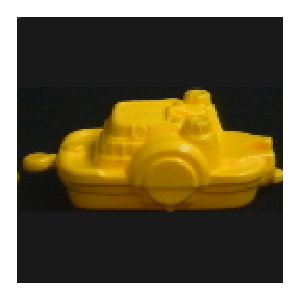
\includegraphics[width=1cm]{coil/beeld-12.eps}
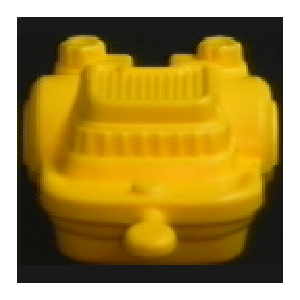
\includegraphics[width=1cm]{coil/beeld-14.eps}
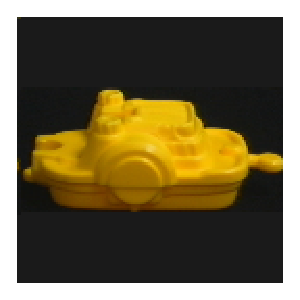
\includegraphics[width=1cm]{coil/beeld-13.eps}
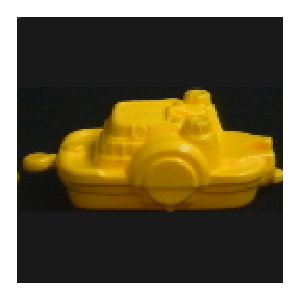
\includegraphics[width=1cm]{coil/beeld-12.eps}
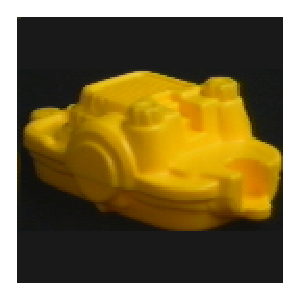
\includegraphics[width=1cm]{coil/beeld-16.eps}
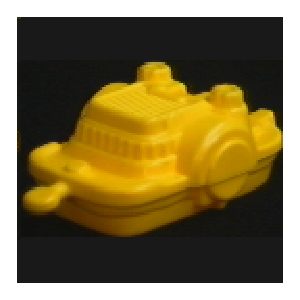
\includegraphics[width=1cm]{coil/beeld-15.eps}

\includegraphics[width=1cm]{coil/beeld-18.eps}
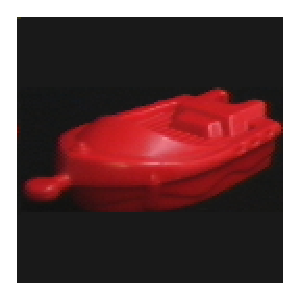
\includegraphics[width=1cm]{coil/beeld-21.eps}
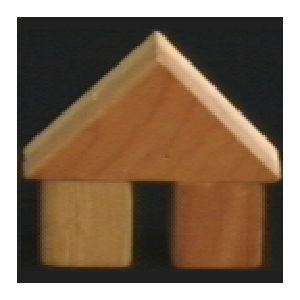
\includegraphics[width=1cm]{coil/beeld-43.eps}
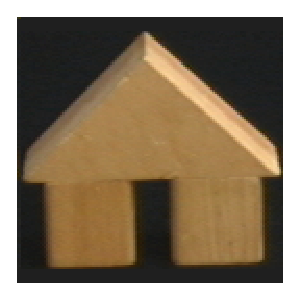
\includegraphics[width=1cm]{coil/beeld-42.eps}
& {\scriptsize 0.0}
\\
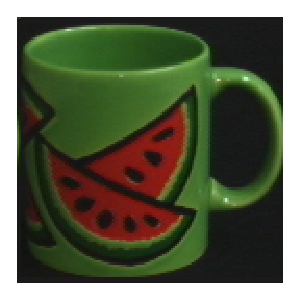
\includegraphics[width=1cm]{coil/beeld-30.eps}
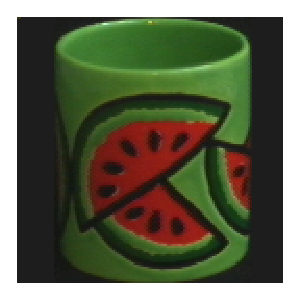
\includegraphics[width=1cm]{coil/beeld-32.eps}
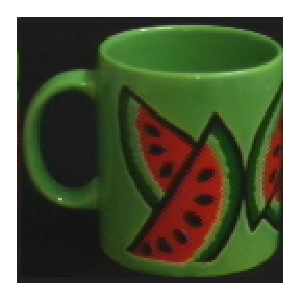
\includegraphics[width=1cm]{coil/beeld-31.eps}
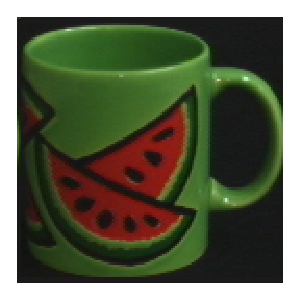
\includegraphics[width=1cm]{coil/beeld-30.eps}
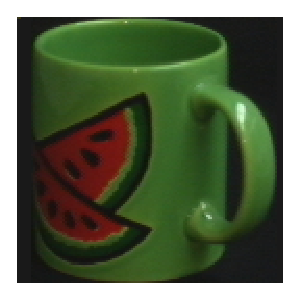
\includegraphics[width=1cm]{coil/beeld-34.eps}
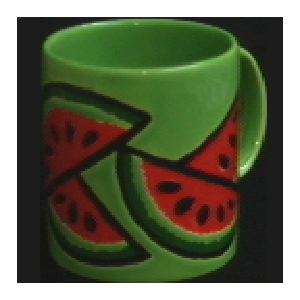
\includegraphics[width=1cm]{coil/beeld-33.eps}
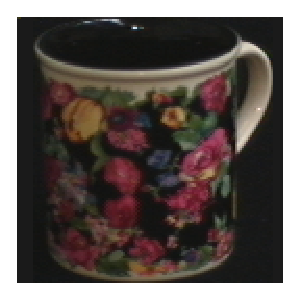
\includegraphics[width=1cm]{coil/beeld-63.eps}
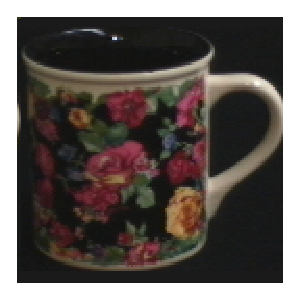
\includegraphics[width=1cm]{coil/beeld-60.eps}
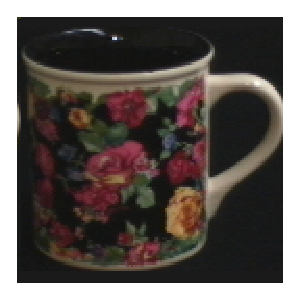
\includegraphics[width=1cm]{coil/beeld-60.eps}

\includegraphics[width=1cm]{coil/beeld-18.eps}
& {\scriptsize 0.0}
\\
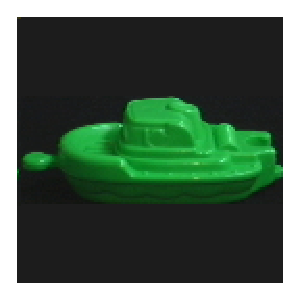
\includegraphics[width=1cm]{coil/beeld-54.eps}
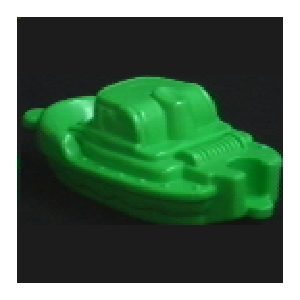
\includegraphics[width=1cm]{coil/beeld-58.eps}
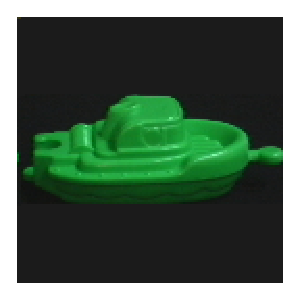
\includegraphics[width=1cm]{coil/beeld-55.eps}
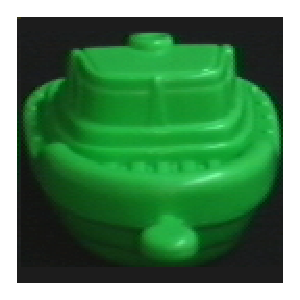
\includegraphics[width=1cm]{coil/beeld-56.eps}
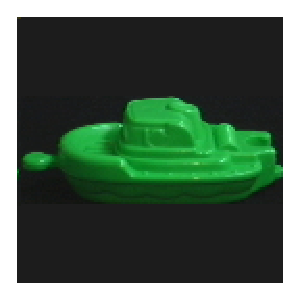
\includegraphics[width=1cm]{coil/beeld-54.eps}
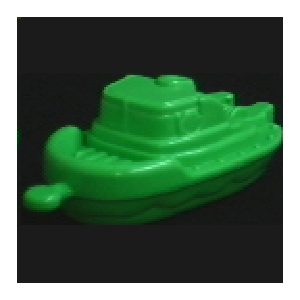
\includegraphics[width=1cm]{coil/beeld-57.eps}
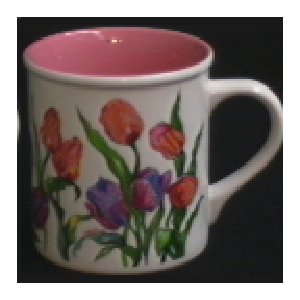
\includegraphics[width=1cm]{coil/beeld-6.eps}
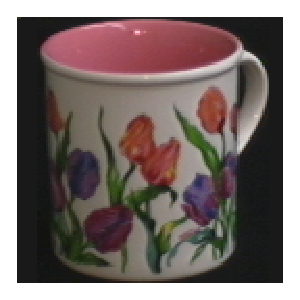
\includegraphics[width=1cm]{coil/beeld-9.eps}
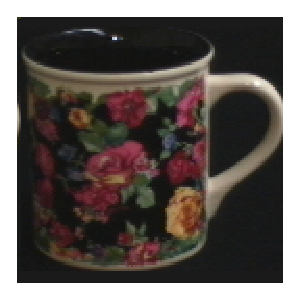
\includegraphics[width=1cm]{coil/beeld-60.eps}
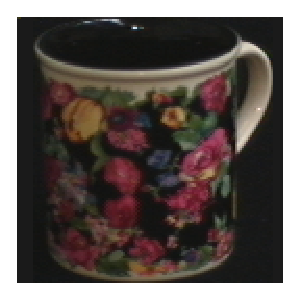
\includegraphics[width=1cm]{coil/beeld-63.eps}
& {\scriptsize 0.0}
\\

\includegraphics[width=1cm]{coil/beeld-18.eps}
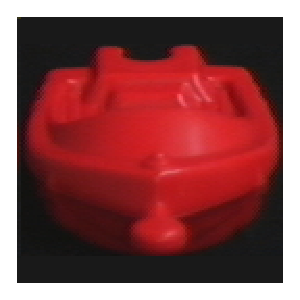
\includegraphics[width=1cm]{coil/beeld-20.eps}
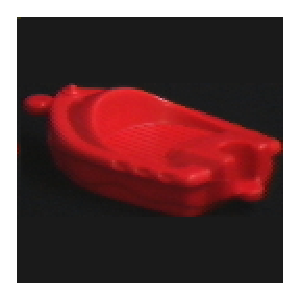
\includegraphics[width=1cm]{coil/beeld-22.eps}

\includegraphics[width=1cm]{coil/beeld-18.eps}
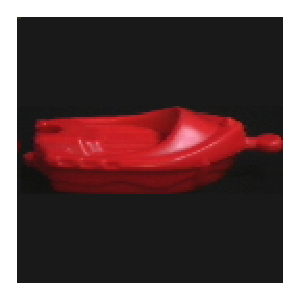
\includegraphics[width=1cm]{coil/beeld-19.eps}
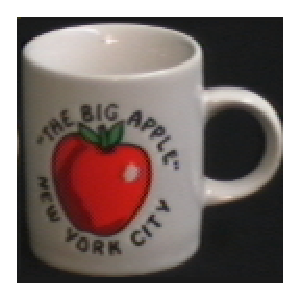
\includegraphics[width=1cm]{coil/beeld-36.eps}
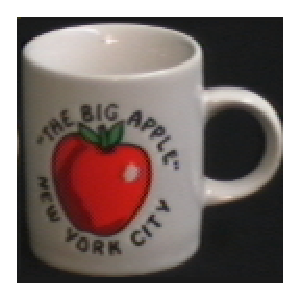
\includegraphics[width=1cm]{coil/beeld-36.eps}
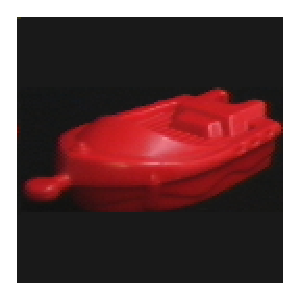
\includegraphics[width=1cm]{coil/beeld-21.eps}
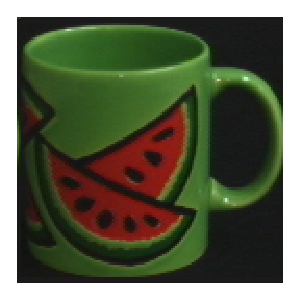
\includegraphics[width=1cm]{coil/beeld-30.eps}
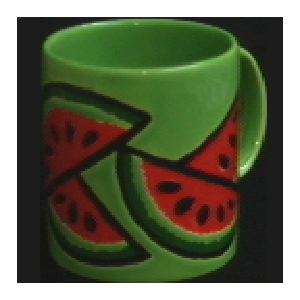
\includegraphics[width=1cm]{coil/beeld-33.eps}
& {\scriptsize 0.004761904761904762}
\\
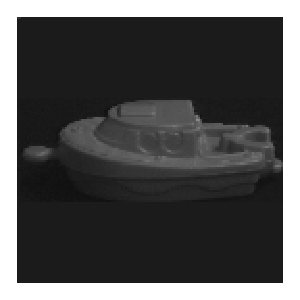
\includegraphics[width=1cm]{coil/beeld-24.eps}
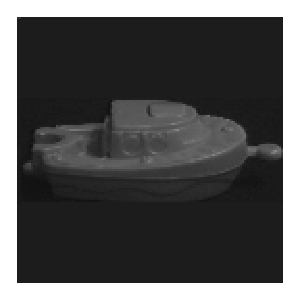
\includegraphics[width=1cm]{coil/beeld-27.eps}
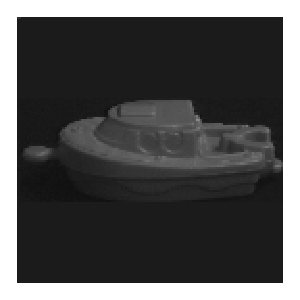
\includegraphics[width=1cm]{coil/beeld-24.eps}
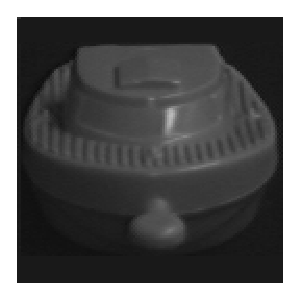
\includegraphics[width=1cm]{coil/beeld-28.eps}
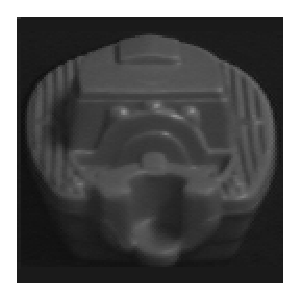
\includegraphics[width=1cm]{coil/beeld-26.eps}
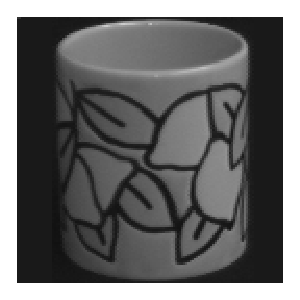
\includegraphics[width=1cm]{coil/beeld-52.eps}
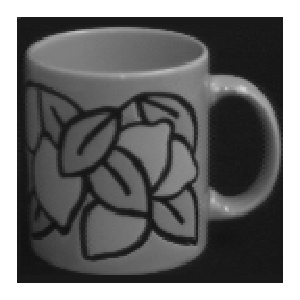
\includegraphics[width=1cm]{coil/beeld-48.eps}
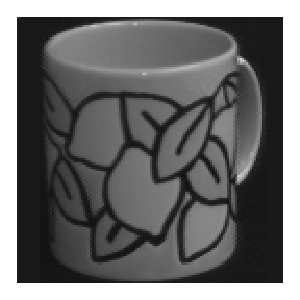
\includegraphics[width=1cm]{coil/beeld-51.eps}
\includegraphics[width=1cm]{coil/beeld-48.eps}
\includegraphics[width=1cm]{coil/beeld-50.eps}
& {\scriptsize 0.014285714285714285}
\\
\includegraphics[width=1cm]{coil/beeld-6.eps}
\includegraphics[width=1cm]{coil/beeld-8.eps}
\includegraphics[width=1cm]{coil/beeld-6.eps}
\includegraphics[width=1cm]{coil/beeld-10.eps}
\includegraphics[width=1cm]{coil/beeld-60.eps}
\includegraphics[width=1cm]{coil/beeld-62.eps}
\includegraphics[width=1cm]{coil/beeld-60.eps}
\includegraphics[width=1cm]{coil/beeld-64.eps}
\includegraphics[width=1cm]{coil/beeld-61.eps}
\includegraphics[width=1cm]{coil/beeld-9.eps}
& {\scriptsize 0.02857142857142857}
\\
\includegraphics[width=1cm]{coil/beeld-60.eps}
\includegraphics[width=1cm]{coil/beeld-60.eps}
\includegraphics[width=1cm]{coil/beeld-6.eps}
\includegraphics[width=1cm]{coil/beeld-9.eps}
\includegraphics[width=1cm]{coil/beeld-64.eps}
\includegraphics[width=1cm]{coil/beeld-39.eps}
\includegraphics[width=1cm]{coil/beeld-36.eps}
\includegraphics[width=1cm]{coil/beeld-63.eps}
\includegraphics[width=1cm]{coil/beeld-43.eps}
\includegraphics[width=1cm]{coil/beeld-62.eps}
& {\scriptsize 0.0380952380952381}
\\
\includegraphics[width=1cm]{coil/beeld-36.eps}
\includegraphics[width=1cm]{coil/beeld-38.eps}
\includegraphics[width=1cm]{coil/beeld-40.eps}
\includegraphics[width=1cm]{coil/beeld-18.eps}
\includegraphics[width=1cm]{coil/beeld-62.eps}
\includegraphics[width=1cm]{coil/beeld-19.eps}
\includegraphics[width=1cm]{coil/beeld-21.eps}
\includegraphics[width=1cm]{coil/beeld-60.eps}
\includegraphics[width=1cm]{coil/beeld-36.eps}
\includegraphics[width=1cm]{coil/beeld-18.eps}
& {\scriptsize 0.05714285714285714}
\\
\includegraphics[width=1cm]{coil/beeld-0.eps}
\includegraphics[width=1cm]{coil/beeld-42.eps}
\includegraphics[width=1cm]{coil/beeld-2.eps}
\includegraphics[width=1cm]{coil/beeld-3.eps}
\includegraphics[width=1cm]{coil/beeld-4.eps}
\includegraphics[width=1cm]{coil/beeld-64.eps}
\includegraphics[width=1cm]{coil/beeld-60.eps}
\includegraphics[width=1cm]{coil/beeld-60.eps}
\includegraphics[width=1cm]{coil/beeld-63.eps}
\includegraphics[width=1cm]{coil/beeld-44.eps}
& {\scriptsize 0.06904761904761905}
\\
\includegraphics[width=1cm]{coil/beeld-24.eps}
\includegraphics[width=1cm]{coil/beeld-27.eps}
\includegraphics[width=1cm]{coil/beeld-25.eps}
\includegraphics[width=1cm]{coil/beeld-24.eps}
\includegraphics[width=1cm]{coil/beeld-28.eps}
\includegraphics[width=1cm]{coil/beeld-26.eps}
\includegraphics[width=1cm]{coil/beeld-48.eps}
\includegraphics[width=1cm]{coil/beeld-50.eps}
\includegraphics[width=1cm]{coil/beeld-49.eps}
\includegraphics[width=1cm]{coil/beeld-48.eps}
& {\scriptsize 0.08571428571428572}
\\
\includegraphics[width=1cm]{coil/beeld-42.eps}
\includegraphics[width=1cm]{coil/beeld-0.eps}
\includegraphics[width=1cm]{coil/beeld-3.eps}
\includegraphics[width=1cm]{coil/beeld-2.eps}
\includegraphics[width=1cm]{coil/beeld-4.eps}
\includegraphics[width=1cm]{coil/beeld-1.eps}
\includegraphics[width=1cm]{coil/beeld-60.eps}
\includegraphics[width=1cm]{coil/beeld-44.eps}
\includegraphics[width=1cm]{coil/beeld-64.eps}
\includegraphics[width=1cm]{coil/beeld-60.eps}
& {\scriptsize 0.20714285714285716}
\end{tabular}
\caption{\label{fig:results_i1i2i3_histgeb}De GGR-waarde en de eerste tien resultaten voor elk voorbeeld-beeld bij de beste I1I2I3-histogram-gebaseerde similariteitsmaat.}
\end{center}
\end{figure}

\begin{figure}[tbp]
\begin{center}
\begin{tabular}{m{11cm} | m{3cm} |}
\textbf{Eerste tien resultaten:} & \textbf{GGR:} \\
\vspace{4pt}
\includegraphics[width=1cm]{coil/beeld-6.eps}
\includegraphics[width=1cm]{coil/beeld-9.eps}
\includegraphics[width=1cm]{coil/beeld-10.eps}
\includegraphics[width=1cm]{coil/beeld-6.eps}
\includegraphics[width=1cm]{coil/beeld-8.eps}
\includegraphics[width=1cm]{coil/beeld-7.eps}
\includegraphics[width=1cm]{coil/beeld-62.eps}
\includegraphics[width=1cm]{coil/beeld-38.eps}
\includegraphics[width=1cm]{coil/beeld-61.eps}
\includegraphics[width=1cm]{coil/beeld-36.eps}
& {\scriptsize 0.0}
\\
\includegraphics[width=1cm]{coil/beeld-30.eps}
\includegraphics[width=1cm]{coil/beeld-31.eps}
\includegraphics[width=1cm]{coil/beeld-34.eps}
\includegraphics[width=1cm]{coil/beeld-33.eps}
\includegraphics[width=1cm]{coil/beeld-30.eps}
\includegraphics[width=1cm]{coil/beeld-32.eps}
\includegraphics[width=1cm]{coil/beeld-42.eps}
\includegraphics[width=1cm]{coil/beeld-16.eps}
\includegraphics[width=1cm]{coil/beeld-60.eps}
\includegraphics[width=1cm]{coil/beeld-60.eps}
& {\scriptsize 0.0}
\\
\includegraphics[width=1cm]{coil/beeld-49.eps}
\includegraphics[width=1cm]{coil/beeld-48.eps}
\includegraphics[width=1cm]{coil/beeld-50.eps}
\includegraphics[width=1cm]{coil/beeld-52.eps}
\includegraphics[width=1cm]{coil/beeld-51.eps}
\includegraphics[width=1cm]{coil/beeld-48.eps}
\includegraphics[width=1cm]{coil/beeld-26.eps}
\includegraphics[width=1cm]{coil/beeld-28.eps}
\includegraphics[width=1cm]{coil/beeld-39.eps}
\includegraphics[width=1cm]{coil/beeld-40.eps}
& {\scriptsize 0.0}
\\
\includegraphics[width=1cm]{coil/beeld-60.eps}
\includegraphics[width=1cm]{coil/beeld-63.eps}
\includegraphics[width=1cm]{coil/beeld-64.eps}
\includegraphics[width=1cm]{coil/beeld-60.eps}
\includegraphics[width=1cm]{coil/beeld-61.eps}
\includegraphics[width=1cm]{coil/beeld-62.eps}
\includegraphics[width=1cm]{coil/beeld-9.eps}
\includegraphics[width=1cm]{coil/beeld-6.eps}
\includegraphics[width=1cm]{coil/beeld-10.eps}
\includegraphics[width=1cm]{coil/beeld-6.eps}
& {\scriptsize 0.0}
\\
\includegraphics[width=1cm]{coil/beeld-12.eps}
\includegraphics[width=1cm]{coil/beeld-15.eps}
\includegraphics[width=1cm]{coil/beeld-12.eps}
\includegraphics[width=1cm]{coil/beeld-13.eps}
\includegraphics[width=1cm]{coil/beeld-16.eps}
\includegraphics[width=1cm]{coil/beeld-42.eps}
\includegraphics[width=1cm]{coil/beeld-14.eps}
\includegraphics[width=1cm]{coil/beeld-31.eps}
\includegraphics[width=1cm]{coil/beeld-49.eps}
\includegraphics[width=1cm]{coil/beeld-50.eps}
& {\scriptsize 0.002380952380952381}
\\
\includegraphics[width=1cm]{coil/beeld-54.eps}
\includegraphics[width=1cm]{coil/beeld-57.eps}
\includegraphics[width=1cm]{coil/beeld-54.eps}
\includegraphics[width=1cm]{coil/beeld-55.eps}
\includegraphics[width=1cm]{coil/beeld-42.eps}
\includegraphics[width=1cm]{coil/beeld-58.eps}
\includegraphics[width=1cm]{coil/beeld-56.eps}
\includegraphics[width=1cm]{coil/beeld-31.eps}
\includegraphics[width=1cm]{coil/beeld-49.eps}
\includegraphics[width=1cm]{coil/beeld-16.eps}
& {\scriptsize 0.004761904761904762}
\\
\includegraphics[width=1cm]{coil/beeld-18.eps}
\includegraphics[width=1cm]{coil/beeld-21.eps}
\includegraphics[width=1cm]{coil/beeld-18.eps}
\includegraphics[width=1cm]{coil/beeld-19.eps}
\includegraphics[width=1cm]{coil/beeld-42.eps}
\includegraphics[width=1cm]{coil/beeld-31.eps}
\includegraphics[width=1cm]{coil/beeld-22.eps}
\includegraphics[width=1cm]{coil/beeld-20.eps}
\includegraphics[width=1cm]{coil/beeld-16.eps}
\includegraphics[width=1cm]{coil/beeld-49.eps}
& {\scriptsize 0.009523809523809525}
\\
\includegraphics[width=1cm]{coil/beeld-36.eps}
\includegraphics[width=1cm]{coil/beeld-36.eps}
\includegraphics[width=1cm]{coil/beeld-38.eps}
\includegraphics[width=1cm]{coil/beeld-37.eps}
\includegraphics[width=1cm]{coil/beeld-40.eps}
\includegraphics[width=1cm]{coil/beeld-8.eps}
\includegraphics[width=1cm]{coil/beeld-7.eps}
\includegraphics[width=1cm]{coil/beeld-6.eps}
\includegraphics[width=1cm]{coil/beeld-9.eps}
\includegraphics[width=1cm]{coil/beeld-39.eps}
& {\scriptsize 0.009523809523809525}
\\
\includegraphics[width=1cm]{coil/beeld-24.eps}
\includegraphics[width=1cm]{coil/beeld-27.eps}
\includegraphics[width=1cm]{coil/beeld-25.eps}
\includegraphics[width=1cm]{coil/beeld-24.eps}
\includegraphics[width=1cm]{coil/beeld-49.eps}
\includegraphics[width=1cm]{coil/beeld-50.eps}
\includegraphics[width=1cm]{coil/beeld-48.eps}
\includegraphics[width=1cm]{coil/beeld-28.eps}
\includegraphics[width=1cm]{coil/beeld-51.eps}
\includegraphics[width=1cm]{coil/beeld-26.eps}
& {\scriptsize 0.016666666666666666}
\\
\includegraphics[width=1cm]{coil/beeld-0.eps}
\includegraphics[width=1cm]{coil/beeld-3.eps}
\includegraphics[width=1cm]{coil/beeld-1.eps}
\includegraphics[width=1cm]{coil/beeld-42.eps}
\includegraphics[width=1cm]{coil/beeld-43.eps}
\includegraphics[width=1cm]{coil/beeld-2.eps}
\includegraphics[width=1cm]{coil/beeld-42.eps}
\includegraphics[width=1cm]{coil/beeld-44.eps}
\includegraphics[width=1cm]{coil/beeld-0.eps}
\includegraphics[width=1cm]{coil/beeld-4.eps}
& {\scriptsize 0.023809523809523808}
\\
\includegraphics[width=1cm]{coil/beeld-42.eps}
\includegraphics[width=1cm]{coil/beeld-0.eps}
\includegraphics[width=1cm]{coil/beeld-3.eps}
\includegraphics[width=1cm]{coil/beeld-1.eps}
\includegraphics[width=1cm]{coil/beeld-43.eps}
\includegraphics[width=1cm]{coil/beeld-2.eps}
\includegraphics[width=1cm]{coil/beeld-0.eps}
\includegraphics[width=1cm]{coil/beeld-42.eps}
\includegraphics[width=1cm]{coil/beeld-4.eps}
\includegraphics[width=1cm]{coil/beeld-44.eps}
& {\scriptsize 0.06190476190476191}
\end{tabular}
\caption{\label{fig:results_irb_histgeb}De GGR-waarde en de eerste tien resultaten voor elk voorbeeld-beeld bij de beste Irb-histogram-gebaseerde similariteitsmaat.}
\end{center}
\end{figure}

\begin{figure}[tbp]
\begin{center}
\begin{tabular}{m{11cm} | m{3cm} |}
\textbf{Eerste tien resultaten:} & \textbf{GGR:} \\
\vspace{4pt}
\includegraphics[width=1cm]{coil/beeld-12.eps}
\includegraphics[width=1cm]{coil/beeld-15.eps}
\includegraphics[width=1cm]{coil/beeld-16.eps}
\includegraphics[width=1cm]{coil/beeld-12.eps}
\includegraphics[width=1cm]{coil/beeld-13.eps}
\includegraphics[width=1cm]{coil/beeld-14.eps}
\includegraphics[width=1cm]{coil/beeld-31.eps}
\includegraphics[width=1cm]{coil/beeld-2.eps}
\includegraphics[width=1cm]{coil/beeld-46.eps}
\includegraphics[width=1cm]{coil/beeld-4.eps}
& {\scriptsize 0.0}
\\
\includegraphics[width=1cm]{coil/beeld-6.eps}
\includegraphics[width=1cm]{coil/beeld-10.eps}
\includegraphics[width=1cm]{coil/beeld-9.eps}
\includegraphics[width=1cm]{coil/beeld-6.eps}
\includegraphics[width=1cm]{coil/beeld-7.eps}
\includegraphics[width=1cm]{coil/beeld-8.eps}
\includegraphics[width=1cm]{coil/beeld-40.eps}
\includegraphics[width=1cm]{coil/beeld-62.eps}
\includegraphics[width=1cm]{coil/beeld-36.eps}
\includegraphics[width=1cm]{coil/beeld-61.eps}
& {\scriptsize 0.0}
\\
\includegraphics[width=1cm]{coil/beeld-31.eps}
\includegraphics[width=1cm]{coil/beeld-30.eps}
\includegraphics[width=1cm]{coil/beeld-33.eps}
\includegraphics[width=1cm]{coil/beeld-30.eps}
\includegraphics[width=1cm]{coil/beeld-34.eps}
\includegraphics[width=1cm]{coil/beeld-32.eps}
\includegraphics[width=1cm]{coil/beeld-56.eps}
\includegraphics[width=1cm]{coil/beeld-58.eps}
\includegraphics[width=1cm]{coil/beeld-16.eps}
\includegraphics[width=1cm]{coil/beeld-54.eps}
& {\scriptsize 0.0}
\\
\includegraphics[width=1cm]{coil/beeld-49.eps}
\includegraphics[width=1cm]{coil/beeld-48.eps}
\includegraphics[width=1cm]{coil/beeld-50.eps}
\includegraphics[width=1cm]{coil/beeld-52.eps}
\includegraphics[width=1cm]{coil/beeld-51.eps}
\includegraphics[width=1cm]{coil/beeld-48.eps}
\includegraphics[width=1cm]{coil/beeld-26.eps}
\includegraphics[width=1cm]{coil/beeld-28.eps}
\includegraphics[width=1cm]{coil/beeld-16.eps}
\includegraphics[width=1cm]{coil/beeld-31.eps}
& {\scriptsize 0.0}
\\
\includegraphics[width=1cm]{coil/beeld-60.eps}
\includegraphics[width=1cm]{coil/beeld-60.eps}
\includegraphics[width=1cm]{coil/beeld-64.eps}
\includegraphics[width=1cm]{coil/beeld-63.eps}
\includegraphics[width=1cm]{coil/beeld-61.eps}
\includegraphics[width=1cm]{coil/beeld-62.eps}
\includegraphics[width=1cm]{coil/beeld-16.eps}
\includegraphics[width=1cm]{coil/beeld-9.eps}
\includegraphics[width=1cm]{coil/beeld-31.eps}
\includegraphics[width=1cm]{coil/beeld-6.eps}
& {\scriptsize 0.0}
\\
\includegraphics[width=1cm]{coil/beeld-36.eps}
\includegraphics[width=1cm]{coil/beeld-37.eps}
\includegraphics[width=1cm]{coil/beeld-38.eps}
\includegraphics[width=1cm]{coil/beeld-40.eps}
\includegraphics[width=1cm]{coil/beeld-36.eps}
\includegraphics[width=1cm]{coil/beeld-7.eps}
\includegraphics[width=1cm]{coil/beeld-6.eps}
\includegraphics[width=1cm]{coil/beeld-9.eps}
\includegraphics[width=1cm]{coil/beeld-8.eps}
\includegraphics[width=1cm]{coil/beeld-10.eps}
& {\scriptsize 0.011904761904761904}
\\
\includegraphics[width=1cm]{coil/beeld-0.eps}
\includegraphics[width=1cm]{coil/beeld-1.eps}
\includegraphics[width=1cm]{coil/beeld-42.eps}
\includegraphics[width=1cm]{coil/beeld-43.eps}
\includegraphics[width=1cm]{coil/beeld-3.eps}
\includegraphics[width=1cm]{coil/beeld-2.eps}
\includegraphics[width=1cm]{coil/beeld-0.eps}
\includegraphics[width=1cm]{coil/beeld-4.eps}
\includegraphics[width=1cm]{coil/beeld-44.eps}
\includegraphics[width=1cm]{coil/beeld-16.eps}
& {\scriptsize 0.01904761904761905}
\\
\includegraphics[width=1cm]{coil/beeld-24.eps}
\includegraphics[width=1cm]{coil/beeld-27.eps}
\includegraphics[width=1cm]{coil/beeld-25.eps}
\includegraphics[width=1cm]{coil/beeld-24.eps}
\includegraphics[width=1cm]{coil/beeld-49.eps}
\includegraphics[width=1cm]{coil/beeld-50.eps}
\includegraphics[width=1cm]{coil/beeld-48.eps}
\includegraphics[width=1cm]{coil/beeld-28.eps}
\includegraphics[width=1cm]{coil/beeld-16.eps}
\includegraphics[width=1cm]{coil/beeld-51.eps}
& {\scriptsize 0.02142857142857143}
\\
\includegraphics[width=1cm]{coil/beeld-54.eps}
\includegraphics[width=1cm]{coil/beeld-57.eps}
\includegraphics[width=1cm]{coil/beeld-55.eps}
\includegraphics[width=1cm]{coil/beeld-54.eps}
\includegraphics[width=1cm]{coil/beeld-31.eps}
\includegraphics[width=1cm]{coil/beeld-16.eps}
\includegraphics[width=1cm]{coil/beeld-56.eps}
\includegraphics[width=1cm]{coil/beeld-14.eps}
\includegraphics[width=1cm]{coil/beeld-32.eps}
\includegraphics[width=1cm]{coil/beeld-0.eps}
& {\scriptsize 0.02857142857142857}
\\
\includegraphics[width=1cm]{coil/beeld-18.eps}
\includegraphics[width=1cm]{coil/beeld-21.eps}
\includegraphics[width=1cm]{coil/beeld-18.eps}
\includegraphics[width=1cm]{coil/beeld-19.eps}
\includegraphics[width=1cm]{coil/beeld-16.eps}
\includegraphics[width=1cm]{coil/beeld-31.eps}
\includegraphics[width=1cm]{coil/beeld-64.eps}
\includegraphics[width=1cm]{coil/beeld-14.eps}
\includegraphics[width=1cm]{coil/beeld-60.eps}
\includegraphics[width=1cm]{coil/beeld-22.eps}
& {\scriptsize 0.030952380952380953}
\\
\includegraphics[width=1cm]{coil/beeld-42.eps}
\includegraphics[width=1cm]{coil/beeld-0.eps}
\includegraphics[width=1cm]{coil/beeld-1.eps}
\includegraphics[width=1cm]{coil/beeld-0.eps}
\includegraphics[width=1cm]{coil/beeld-4.eps}
\includegraphics[width=1cm]{coil/beeld-2.eps}
\includegraphics[width=1cm]{coil/beeld-43.eps}
\includegraphics[width=1cm]{coil/beeld-3.eps}
\includegraphics[width=1cm]{coil/beeld-46.eps}
\includegraphics[width=1cm]{coil/beeld-44.eps}
& {\scriptsize 0.07142857142857142}
\end{tabular}
\caption{\label{fig:results_yxy_histgeb}De GGR-waarde en de eerste tien resultaten voor elk voorbeeld-beeld bij de beste Yxy-histogram-gebaseerde similariteitsmaat.}
\end{center}
\end{figure}


% \subsection{Histogram smoothing}


\subsection{Vaaghistogram}

Naast de bovenstaande vage interpretatie van het klassieke kleurhistogram, beschouwen we
ook nog een gelijkaardige kleurbeschrijving die we op een ``volledig vage'' manier opbouwen. Bij dit
\emph{vaaghistogram} maken we gebruik van het (niet genormaliseerde) L*a*b* kleurmodel en 
beschouwen we een vaagverzameling voor elke kleur. 
De lidmaatschapsgraad van een kleur $c'$ in de vaagverzameling 
$FC_c$, die correspondeert met kleur $c$, defini\"eren we als volgt \cite{vertan:fuzzy_histograms}: 
$$
\begin{array}{rcll}
FC_c(c') & = & 1 & \textrm{als } d(c,c') \leq 2.3 \\
		 & = & \exp \left( - \frac{\left((d(c,c') / 2.3) - 1\right)^2}{2 \cdot \lambda^2} \right) & \textrm{anders}
\end{array}
$$  
met $d$ de Euclidische afstand en $\lambda$ een vrij te kiezen parameter, die we in deze scriptie
voor de eenvoud steeds gelijk aan $1$ zullen kiezen. In het geval van L*a*b* 
komt de afstand $2.3$ namelijk overeen met de zogenaamde \emph{just noticeable difference} (JND)
\cite{sharma:digital_color_imaging}. 
Kleuren waarvan de onderlinge afstand kleiner dan of gelijk aan deze JND is, kunnen door de mens 
niet onderscheiden worden.

Het eigenlijk vaaghistogram $Fh_A$, voor een kleurbeeld $A$, defini\"eren we dan als de unie van 
alle kleuren die voorkomen in $A$:
$$
Fh_A = \displaystyle\bigcup_{c \in C_A} FC_c
%\begin{array}{lrcl}
%Fh_A: 	& C_A 	& \to 		& [0,1] \\[5pt]
%		& c					& \mapsto	& \displaystyle\bigcup_{c \in C_A} FC_c,
%\quad\forall c \in C_A
%\end{array}
$$ 
waarbij de verzameling $C_A$ bestaat uit de in $A$ voorkomende kleuren.

\subsubsection{Experimentele observaties}